\documentclass{beamer}
\usetheme{Madrid}
\usecolortheme{whale}
\usepackage{tikz}
\usepackage{amsmath}
\usetikzlibrary{arrows,shapes,positioning,shadows,trees}

\title{Philosophy of Race: Ethical Perspectives}
\author{Brendan Shea, PhD}
\date{Introduction to Ethics}

\begin{document}
	
	\begin{frame}
		\titlepage
	\end{frame}
	
	\begin{frame}{Ethics and Race: An Introduction to Critical Concepts}
		\begin{itemize}
			\item Philosophy of race examines the meaning, significance, and ethical implications of racial categories and racial identity.
			\item The field connects metaphysics (what race is) with ethics (how we should respond to racial realities).
			\item Race raises fundamental questions about justice, fairness, and human dignity that are central to ethical inquiry.
			\item Understanding race philosophically helps us evaluate policies and practices intended to address racial inequality.
		\end{itemize}
		
		\begin{alertblock}{Key Question}
			How does race shape our moral obligations to one another in society?
		\end{alertblock}
	\end{frame}
	
	\begin{frame}{What is Race? Biological Concepts vs. Social Construction}
		\begin{itemize}
			\item \textbf{Biological race}: The theory that humans can be divided into distinct groups with inherited physical and behavioral characteristics. 
			\item Modern genetic science has rejected traditional biological concepts, since race doesn't track genetic difference. Some modern views of race still posit a role for ancestry. 
			\item \textbf{Social construction} refers to the idea that race is created through social practices and institutions rather than biology.
			\item \textbf{Racial nominalism} (or "racial anti-realism") holds that there is no single, coherent concepts of race by the standards of the either the biological or social sciences. Race is a "fiction" that has often been used to harm people. 
		\end{itemize}
		
	\end{frame}
	
	\begin{frame}{Racialism and Racism: Defining Core Terminology}
		\begin{itemize}
			\item \textbf{Racialism} is the belief that humans can be divided into distinct racial groups with inherited characteristics.
			\item \textbf{Racism} involves prejudice, discrimination, or antagonism based on racial categorization, typically with power dynamics.
			\item \textbf{Institutional racism} refers to racial discrimination embedded in laws, policies, and practices of social institutions.
			\item \textbf{Structural racism} describes how historical, cultural, and social patterns create disadvantages for certain racial groups.
		\end{itemize}
		
		\begin{exampleblock}{Example: Redlining}
			Redlining was a discriminatory practice where financial institutions refused services to residents of certain areas based on racial composition, demonstrating institutional racism with long-term structural effects.
		\end{exampleblock}
	\end{frame}
	
	\begin{frame}{Race as a Historical Phenomenon: Origins and Evolution}
		\begin{itemize}
			\item Modern racial categories emerged primarily during European colonization and the transatlantic slave trade.
			\item Racial classifications have changed significantly across time and place, demonstrating their contingent nature.
			\item In the US, beliefs about who is "white" has expanded over time to include previously excluded groups like Irish-, Italian-, Jewish-, or Slavic-Americans.
		\end{itemize}
		
		\begin{block}{Timeline of Racial Thinking}
			\begin{tabular}{|l|l|}
				\hline
				\textbf{Period} & \textbf{Development} \\
				\hline
				15th-16th C & Early European colonization and slave trade \\
				17th-18th C & Scientific racism and Enlightenment \\
				19th C & Height of scientific racism and eugenics \\
				20th C & Critique of biological race; civil rights \\
				\hline
			\end{tabular}
		\end{block}
	\end{frame}
	
	\begin{frame}{Philosophical Approaches to Understanding Race}
		\begin{itemize}
			\item \textbf{Racial skepticism} holds that race is an illusion and should be eliminated from our thinking.
			\item \textbf{Racial constructionism} acknowledges race as socially real while rejecting biological essentialism.
			\item \textbf{Racial eliminativism} argues we should abandon racial categories entirely as harmful fictions.
			\item \textbf{Racial conservationism} suggests we should preserve certain aspects of racial identity for positive purposes.
		\end{itemize}
		
		\begin{center}
			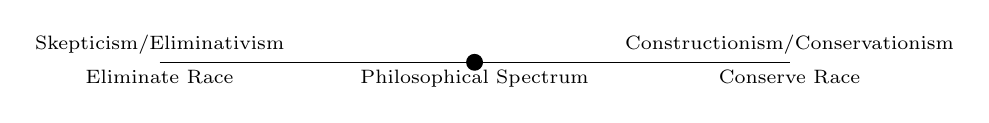
\begin{tikzpicture}
				\scriptsize
				\draw (-4,0) -- (4,0);
				\draw (-4,0) node[below] {Eliminate Race} node[above] {Skepticism/Eliminativism};
				\draw (4,0) node[below] {Conserve Race} node[above] {Constructionism/Conservationism};
				\draw[fill=black] (0,0) circle (0.1) node[below] {Philosophical Spectrum};
			\end{tikzpicture}
		\end{center}
	\end{frame}
	
	\begin{frame}{The Ethics of Racial Categories: Who Decides and Why?}
		\begin{itemize}
			\item Racial classifications have historically been imposed by dominant groups for purposes of control and exploitation.
			\item Self-identification allows individuals autonomy but raises questions about the limits of racial identity claims.
			\item Government classification systems (like the U.S. Census) have real consequences for resource allocation and representation.
			\item The ethics of classification involves balancing respect for identity with the need to address historical injustices.
		\end{itemize}
		
		\begin{block}{Ethical Principles at Stake}
			\begin{itemize}
				\item Autonomy: Right to self-definition
				\item Justice: Addressing historical wrongs
				\item Utility: Practical benefits of categories
				\item Recognition: Respecting identity claims
			\end{itemize}
		\end{block}
	\end{frame}
	
	\begin{frame}{Race in Revolutionary America: Liberty and Contradiction}
		\begin{itemize}
			\item America's founding documents proclaimed universal principles of freedom while maintaining racial slavery.
			\item The contradiction between "all men are created equal" and racialized slavery created philosophical tension.
			\item Thinkers like Thomas Jefferson simultaneously advocated liberty while owning slaves and promoting racial hierarchy.
			\item This founding contradiction established a pattern of racial paradox that continues in American ethical life.
		\end{itemize}
		
		\begin{exampleblock}{Jefferson's Paradox}
			In his \textit{Notes on the State of Virginia} (1785), Jefferson articulated natural rights philosophy while also arguing for Black inferiority—demonstrating how Enlightenment thinkers rationalized racial hierarchy while advocating universal liberty.
		\end{exampleblock}
	\end{frame}
	
	\begin{frame}{Slavery, Emancipation, and Reconstruction: Moral Frameworks}
		\begin{itemize}
			\item Proslavery arguments combined religious, economic, paternalistic, and pseudo-scientific justifications for racial bondage.
			\item Abolitionist philosophy appealed to natural rights, religious equality, and universal moral principles.
			\item Reconstruction (1865-1877) represented America's first attempt to create a multiracial democracy based on equality.
			\item The (partial) failure of Reconstruction demonstrates how moral progress on race can be reversed by political retrenchment.
		\end{itemize}
		
		\begin{alertblock}{Competing Ethical Frameworks: 19th Century}
			\begin{tabular}{|l|l|}
				\hline
				\textbf{Proslavery Ethics} & \textbf{Abolitionist Ethics} \\
				\hline
				Racial Hierarchy & Natural rights \\
				Preservation of status quo & Right to revolution\\
				Divine ``approval'' for slavery & Religious equality (imago dei) \\
				\hline
			\end{tabular}
		\end{alertblock}
	\end{frame}
	
	\begin{frame}{Jim Crow America: Segregation as Political Philosophy}
		\begin{itemize}
			\item Jim Crow laws (1877-1965) established a comprehensive system of racial separation and subordination.
			\item \textbf{Separate but equal} doctrine in \textit{Plessy v. Ferguson} (1896) provided the legal foundation for segregation.
			\item Segregation was justified through a political philosophy that viewed racial separation as natural and necessary.
			\item This period shows how law and philosophy can work together to codify and naturalize racial hierarchy.
		\end{itemize}
		
		\begin{exampleblock}{The Racial Contract}
			Philosopher Charles Mills argues that racial hierarchy functions as an implicit "racial contract" where white supremacy operates as a political system that structures society while presenting itself as neutral and natural.
		\end{exampleblock}
	\end{frame}
	
	\begin{frame}{Civil Rights Movement: Philosophical Underpinnings}
		\begin{itemize}
			\item The civil rights movement combined diverse philosophical traditions to challenge segregation and discrimination.
			\item \textbf{Natural law} arguments appealed to universal moral principles above unjust human laws.
			\item \textbf{American civic ideals} were invoked to hold the nation accountable to its own stated principles.
			\item The movement demonstrated how philosophical ideas can mobilize social action and legislative change.
		\end{itemize}
		
		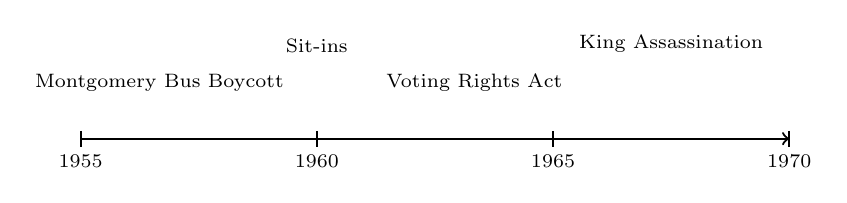
\begin{tikzpicture}
			\scriptsize
			\draw [thick, ->] (0,0) -- (9,0);
			\foreach \x/\t in {0/1955, 3/1960, 6/1965, 9/1970}
			\draw[thick] (\x,0.1) -- (\x,-0.1) node[below] {\t};
			\node[above] at (1,0.5) {Montgomery Bus Boycott};
			\node[above] at (3,1) {Sit-ins};
			\node[above] at (5,0.5) {Voting Rights Act};
			\node[above] at (7.5,1) {King Assassination};
		\end{tikzpicture}
	\end{frame}
	
	\begin{frame}{W.E.B. Du Bois's Life and Intellectual Development}
		\begin{itemize}
			\item William Edward Burghardt Du Bois (1868-1963) was the first African American to earn a PhD from Harvard (1895).
			\item Du Bois combined empirical social science with philosophical analysis to challenge prevailing racial theories.
			\item His intellectual journey moved from liberal reform to more radical critique of capitalism and imperialism.
			\item Du Bois's 95-year lifespan allowed him to witness and analyze radical transformations in American racial dynamics.
		\end{itemize}
		
		\begin{alertblock}{Key Intellectual Periods}
			\begin{itemize}
				\item Academic (1895-1910): Empirical studies challenging racist science
				\item NAACP (1910-1934): Civil rights activism and public intellectual work
				\item Return to Academia (1934-1944): Historical and theoretical writing
				\item Radical Period (1944-1963): Pan-Africanism and global analysis
			\end{itemize}
		\end{alertblock}
	\end{frame}
	
	\begin{frame}{Double Consciousness: Philosophical Analysis}
		\begin{itemize}
			\item \textbf{Double consciousness} is Du Bois's concept describing the "sense of always looking at one's self through the eyes of others."
			\item This concept addresses how racism creates a divided experience of identity for Black Americans.
			\item Double consciousness involves both the burden of "two-ness" and the potential resource of multiple perspectives.
			\item The concept connects epistemology (how we know) with identity formation and social philosophy.
		\end{itemize}
		
		\begin{block}{From The Souls of Black Folk (1903)}
			``It is a peculiar sensation, this double-consciousness, this sense of always looking at one’s self through the eyes of others, of measuring one’s soul by the tape of a world that looks on in amused contempt and pity. One ever feels his two-ness,—an American, a Negro; two souls, two thoughts, two unreconciled strivings; two warring ideals in one dark body, whose dogged strength alone keeps it from being torn asunder.''
		\end{block}
	\end{frame}
	
	\begin{frame}{The Souls of Black Folk: Key Arguments and Frameworks}
		\begin{itemize}
			\item Published in 1903, \textit{The Souls of Black Folk} combines sociology, history, memoir, and philosophy.
			\item The work critiques Booker T. Washington's accommodationist approach to race relations.
			\item Du Bois introduces the concept of the \textbf{"Veil"} to describe how race separates and obscures human understanding.
			\item The book establishes Du Bois's argument that the "problem of the color line" is the central question of the 20th century.
		\end{itemize}
		
		\begin{exampleblock}{The Veil as Philosophical Concept}
			The Veil represents both social separation and epistemic limitation—racial division prevents full human recognition and understanding across racial lines, creating different lived realities.
		\end{exampleblock}
	\end{frame}
	
	\begin{frame}{Du Bois on Education: The Talented Tenth and Beyond}
		\begin{itemize}
			\item \textbf{"The Talented Tenth"} (1903) argues that advanced education for exceptional Black individuals is necessary for racial progress.
			\item Du Bois opposed purely industrial education, advocating for liberal arts education to develop leaders and critical thinkers.
			\item His educational philosophy emphasized that full citizenship requires cultural and intellectual development, not just economic skills.
			\item Later in life, Du Bois revised this elitist approach, emphasizing broader democratic education for all.
		\end{itemize}

	\end{frame}
	
	\begin{frame}{Du Bois's Critique of American Capitalism and Democracy}
		\begin{itemize}
			\item Du Bois argued that racism is fundamentally connected to economic exploitation under capitalism.
			\item In \textit{Black Reconstruction in America} (1935), he reinterpreted the Civil War and Reconstruction through a materialist lens.
			\item He identified the psychological \textbf{wages of whiteness} that prevented class solidarity across racial lines.
			\item Du Bois's analysis connects race, class, and democracy, showing how racial division undermines democratic potential.
		\end{itemize}
		
		\begin{block}{Key Theoretical Innovation}
			Du Bois blended Marxist analysis with his earlier arguments about race, arguing that racial capitalism creates unique forms of exploitation that cannot be reduced to either race or class alone—anticipating contemporary intersectional approaches.
		\end{block}
	\end{frame}
	
	\begin{frame}{Pan-Africanism: Du Bois's Global Philosophy}
		\begin{itemize}
			\item \textbf{Pan-Africanism} argues for the unity and solidarity of African peoples worldwide based on shared historical experiences.
			\item Du Bois organized multiple Pan-African Congresses (1919-1945) to advance anticolonial movements.
			\item He connected racism in America with European colonialism in Africa and Asia as part of a global system of racial hierarchy.
			\item This global perspective reframes race as an international phenomenon requiring transnational solutions.
		\end{itemize}
		
		\begin{tabular}{|l|l|l|}
			\hline
			\textbf{Congress} & \textbf{Year} & \textbf{Key Focus} \\
			\hline
			First Pan-African & 1919 & Post-WWI self-determination \\
			Second Pan-African & 1921 & Economic cooperation \\
			Fifth Pan-African & 1945 & Anticolonialism \\
			\hline
		\end{tabular}
	\end{frame}
	
	\begin{frame}{Du Bois's Later Works: Evolving Thought on Race and Justice}
		\begin{itemize}
			\item In his final decades, Du Bois increasingly embraced socialism as necessary for racial justice.
			\item \textit{Dusk of Dawn} (1940) offers an "autobiography of a concept of race," connecting personal experience with philosophical analysis.
			\item Du Bois became more critical of American liberalism, seeing its limits in addressing deep racial and economic inequality.
			\item He emigrated to Ghana in 1961, symbolically rejecting American racism and embracing Pan-African solidarity.
		\end{itemize}
		
		\begin{alertblock}{Intellectual Evolution}
			Du Bois's seven-decade career demonstrates how philosophical thinking on race can evolve in response to historical events, intellectual engagement, and personal experience—from reform-minded liberalism to revolutionary critique.
		\end{alertblock}
	\end{frame}
	
	\begin{frame}{King's Philosophical Influences: Personalism and Natural Law}
		\begin{itemize}
			\item Martin Luther King Jr. (1929-1968) developed a philosophical framework synthesizing multiple traditions.
			\item \textbf{Personalism}, studied during his Boston University doctorate, emphasizes the inherent dignity and worth of all persons.
			\item \textbf{Natural law} theory provided King with a basis for distinguishing just from unjust laws.
			\item King integrated Christian theology, Gandhian nonviolence, and American democratic ideals into a coherent philosophy.
		\end{itemize}
		
		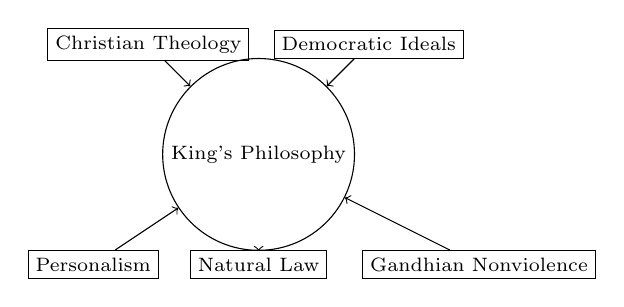
\begin{tikzpicture}[scale = .7]
			\scriptsize
			\node (king) at (4,3) [draw, circle, minimum size=1.5cm] {King's Philosophy};
			\node (personalism) at (1,1) [draw, rectangle] {Personalism};
			\node (natural) at (4,1) [draw, rectangle] {Natural Law};
			\node (gandhi) at (8,1) [draw, rectangle] {Gandhian Nonviolence};
			\node (theology) at (2,5) [draw, rectangle] {Christian Theology};
			\node (democracy) at (6,5) [draw, rectangle] {Democratic Ideals};
			
			\draw [->] (personalism) -- (king);
			\draw [->] (natural) -- (king);
			\draw [->] (gandhi) -- (king);
			\draw [->] (theology) -- (king);
			\draw [->] (democracy) -- (king);
		\end{tikzpicture}
	\end{frame}
	
	\begin{frame}{King on Civil Disobedience: Moral and Philosophical Justifications}
		\begin{itemize}
			\item King defined \textbf{civil disobedience} as breaking unjust laws openly, lovingly, and with willingness to accept consequences.
			\item He distinguished between just and unjust laws using natural law principles and the Personalist emphasis on human dignity.
			\item Unjust laws, for King, are those that degrade human personality or are imposed without representation.
			\item King's theory connects individual conscience with community responsibility, creating an ethics of resistance.
		\end{itemize}
		
		\begin{block}{From "Letter from Birmingham Jail" (1963)}
			"An unjust law is a code that a numerical or power majority group compels a minority group to obey but does not make binding on itself. This is difference made legal. By the same token, a just law is a code that a majority compels a minority to follow and that it is willing to follow itself. This is sameness made legal."
		\end{block}
	\end{frame}
	
	\begin{frame}{The "Beloved Community": Philosophical Foundations}
		\begin{itemize}
			\item \textbf{The Beloved Community} represents King's vision of a just society based on love, integration, and shared prosperity.
			\item This concept is grounded in Personalism's respect for the inherent worth and dignity of every individual.
			\item King rejected both segregation and superficial integration, advocating for genuine interrelatedness across racial lines.
			\item The Beloved Community represents a teleological ethical framework—a moral end toward which social action should aim.
		\end{itemize}
		
		\begin{exampleblock}{Three Dimensions of the Beloved Community}
			\begin{itemize}
				\item \textbf{Integration}: Beyond mere desegregation to genuine community
				\item \textbf{Economic Justice}: Shared prosperity and material wellbeing
				\item \textbf{Reconciliation}: Healing historical wounds through love and forgiveness
			\end{itemize}
		\end{exampleblock}
	\end{frame}
	
	\begin{frame}{King's Philosophy of Nonviolence: Ethical Frameworks}
		\begin{itemize}
			\item King's nonviolence is not merely tactical but based on profound ethical principles about human interrelationship.
			\item \textbf{Agape love}—selfless, unconditional love seeking another's good—forms the spiritual foundation of nonviolent resistance.
			\item Nonviolence aims to defeat injustice without defeating the person, preserving the possibility of reconciliation.
			\item This approach rejects both passive acceptance and violent resistance in favor of a "third way" of creative tension.
		\end{itemize}
		
		\begin{alertblock}{The Six Principles of Nonviolence}
			\scriptsize
			\begin{enumerate}
				\item Nonviolence is a way of life for courageous people
				\item Nonviolence seeks to win friendship and understanding
				\item Nonviolence seeks to defeat injustice, not people
				\item Nonviolence holds that suffering can educate and transform
				\item Nonviolence chooses love instead of hate
				\item Nonviolence believes that the universe is on the side of justice
			\end{enumerate}
		\end{alertblock}
	\end{frame}
	
	\begin{frame}{Letter from Birmingham Jail: Philosophical Analysis}
		\begin{itemize}
			\item Written in April 1963, the letter responds to white clergymen who criticized civil rights demonstrations as "unwise and untimely."
			\item King develops a sophisticated argument for civil disobedience based on natural law, religious ethics, and democratic principles.
			\item The letter articulates the moral imperative of \textbf{direct action} to create productive tension that forces negotiation.
			\item King challenges the \textbf{myth of time} arguing that ``justice delayed is justice denied'', and critiques white moderates' preference for order over justice.
		\end{itemize}
		
		\begin{block}{Key Philosophical Moves}
			The letter demonstrates King's ability to connect abstract philosophical principles with concrete social realities, making moral philosophy immediately relevant to contemporary political struggles.
		\end{block}
	\end{frame}
	
	\begin{frame}{King's Critique of Moderate Liberalism}
		\begin{itemize}
			\item King identified the \textbf{white moderate} as a greater obstacle to justice than the explicit racist due to preference for order over justice.
			\item He criticized gradualism as a form of moral evasion that preserves injustice while claiming to support change.
			\item King challenged proceduralism that prioritizes proper channels over moral urgency in addressing fundamental rights.
			\item This critique reveals the limitations of liberal approaches to racial justice that fail to recognize the moral emergency of racism.
		\end{itemize}
		
		\begin{exampleblock}{From Letter from Birmingham Jail}
			"I have almost reached the regrettable conclusion that the Negro's great stumbling block in his stride toward freedom is not the White Citizen's Counciler or the Ku Klux Klanner, but the white moderate, who is more devoted to 'order' than to justice; who prefers a negative peace which is the absence of tension to a positive peace which is the presence of justice."
		\end{exampleblock}
	\end{frame}
	
	\begin{frame}{Beyond Race: King's Later Philosophy on Poverty and War}
		\begin{itemize}
			\item In his final years (1965-1968), King expanded his critique to address interconnected forms of injustice beyond racial segregation.
			\item The Poor People's Campaign targeted economic inequality across racial lines as a fundamental ethical issue.
			\item King's opposition to the Vietnam War connected militarism, racism, and materialism as \textbf{triple evils} threatening human flourishing.
			\item This broader vision reflects King's development toward a more radical critique of American society and global systems.
		\end{itemize}
		
		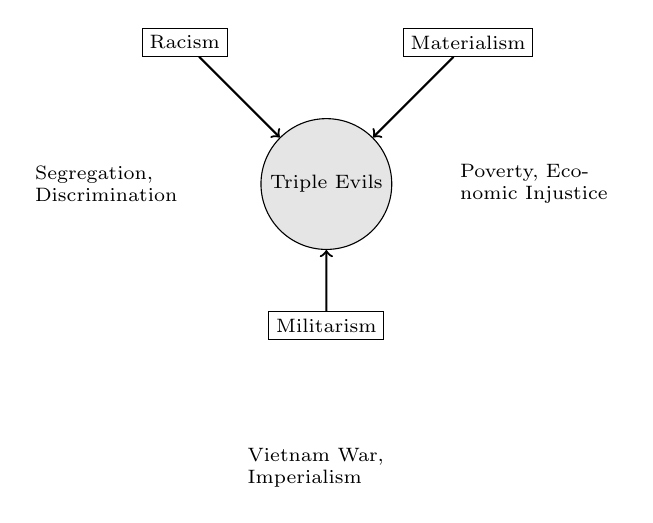
\begin{tikzpicture}[scale = .9]
			\scriptsize
			\node[draw, circle, fill=gray!20] (triple) at (4,2) {Triple Evils};
			\node[draw] (racism) at (2,4) {Racism};
			\node[draw] (materialism) at (6,4) {Materialism};
			\node[draw] (militarism) at (4,0) {Militarism};
			
			\draw[thick, ->] (racism) -- (triple);
			\draw[thick, ->] (materialism) -- (triple);
			\draw[thick, ->] (militarism) -- (triple);
			
			\node[text width=2cm] at (1,2) {Segregation, Discrimination};
			\node[text width=2cm] at (7,2) {Poverty, Economic Injustice};
			\node[text width=2cm] at (4,-2) {Vietnam War, Imperialism};
		\end{tikzpicture}
	\end{frame}
	
	\begin{frame}{Appiah's Life and Intellectual Context}
		\begin{itemize}
			\item Kwame Anthony Appiah (b. 1954) was born in London to a Ghanaian father and English mother, giving him a cross-cultural perspective.
			\item His education at Cambridge and work at institutions like Harvard, Princeton, and NYU places him within Anglo-American analytic philosophy.
			\item Appiah's personal experience as a gay, biracial, transnational intellectual informs his approach to identity questions.
			\item He emerged as a key figure in post-colonial thought while also engaging with traditional analytic philosophy's concerns.
		\end{itemize}
		
		\begin{alertblock}{Intellectual Evolution}
			Unlike Du Bois and King who worked primarily as activists and public intellectuals, Appiah has developed his ideas primarily within academic philosophy, bringing analytical rigor to questions of race and identity.
		\end{alertblock}
	\end{frame}
	
	\begin{frame}{In My Father's House: Key Arguments on African Identity}
		\begin{itemize}
			\item \textit{In My Father's House} (1992) critically examines concepts of African identity and Pan-Africanism.
			\item Appiah argues that many claims about "African" identity or culture rely on problematic essentialist assumptions.
			\item He traces how Western racial concepts have been internalized within African thought, creating distorted self-understandings.
			\item The book demonstrates the ethical importance of historical accuracy in constructing cultural identities.
		\end{itemize}
		
		\begin{block}{On Pan-Africanism and Identity}
			Appiah shows how Pan-Africanism, while politically useful in anti-colonial struggles, often relies on the same racial essentialist thinking developed by European racism—demonstrating how resistance can inadvertently reinforce problematic categories.
		\end{block}
	\end{frame}
	
	\begin{frame}{The Ethics of Identity: Philosophical Framework}
		\begin{itemize}
			\item In \textit{The Ethics of Identity} (2005), Appiah develops a liberal individualist approach to identity questions.
			\item He argues that \textbf{identities} (e.g., race, religion, gender, nationality etc.) provide "scripts" that help us make sense of our lives and choices.
			\item \textbf{Rooted cosmopolitanism} acknowledges the value of cultural roots while emphazing that the moral community includes ALL people (regardless of things like national boundaries).
			\item Appiah seeks a balance between recognizing collective identity and preserving individual autonomy.
		\end{itemize}
		\end{frame}
	
	\begin{frame}{Appiah's Critique of Racial Essentialism}
		\begin{itemize}
			\item \textbf{Racial essentialism} is the belief that racial groups share inherent, defining properties that determine identity and behavior.
			\item Appiah argues that races do not have biological essences and that cultural or historical essences are equally problematic.
			\item He distinguishes between racial identity (how one identifies) and racial classification (how one is categorized by others).
			\item This anti-essentialist position challenges both racist thought and some forms of identity politics that reify racial categories.
		\end{itemize}
		
		\begin{exampleblock}{Philosophical Position}
			Appiah advocates \textbf{racial nominalism}—the view that races are labels without corresponding essences—while acknowledging that these labels have real social effects that cannot be ignored simply because race is not biologically real.
		\end{exampleblock}
	\end{frame}
	
	\begin{frame}{Cosmopolitanism: Theoretical Foundations}
		\begin{itemize}
			\item \textbf{Cosmopolitanism} in Appiah's work refers to the ethical stance that we have obligations to those beyond our immediate community.
			\item In \textit{Cosmopolitanism: Ethics in a World of Strangers} (2006), he balances universal concern with respect for legitimate cultural differences.
			\item Appiah rejects both rigid cultural relativism and imposed universalism in favor of cross-cultural conversation.
			\item This position places Appiah in dialogue with liberal political philosophy while extending it to address global ethics.
		\end{itemize}
		
		\begin{block}{Two Strands of Cosmopolitanism}
			\begin{itemize}
				\item \textbf{Universal concern}: Obligation to value human life across cultural boundaries
				\item \textbf{Respect for difference}: Recognition of legitimate cultural variation without requiring uniformity
			\end{itemize}
		\end{block}
	\end{frame}
	
	\begin{frame}{Ethics Beyond Borders: Appiah on Global Justice}
		\begin{itemize}
			\item Appiah develops a moderate cosmopolitanism that acknowledges special obligations to those nearest to us.
			\item He argues that global ethical responsibilities do not require abandoning particular identities and affiliations.
			\item Cosmopolitan ethics requires both respecting cultural differences and identifying universal harms that cross cultural lines.
			\item This approach offers a middle path between universalism that ignores difference and relativism that abandons shared ethical standards.
		\end{itemize}
     \begin{center}
	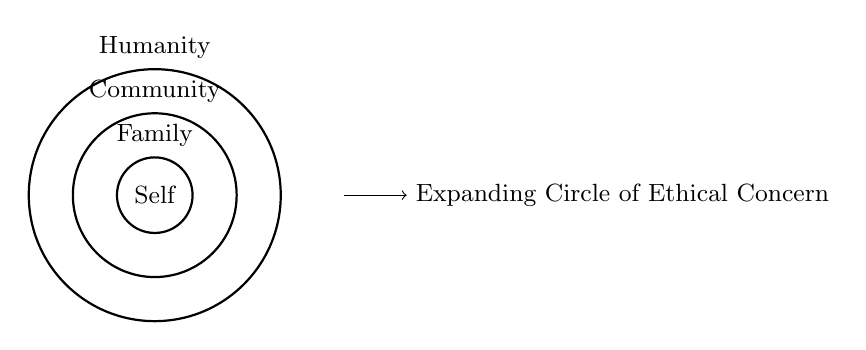
\begin{tikzpicture}[scale = 0.8]
		\small
		\draw [thick] (0,0) circle (2cm);
		\draw [thick] (0,0) circle (1.3cm);
		\draw [thick] (0,0) circle (0.6cm);
		\node at (0,0) {Self};
		\node at (0,0.95) {Family};
		\node at (0,1.65) {Community};
		\node at (0,2.35) {Humanity};
		\draw [->] (3,0) -- (4,0);
		\node [right] at (4,0) {Expanding Circle of Ethical Concern};
	\end{tikzpicture}
\end{center}

	\end{frame}
	
	\begin{frame}{Honor Ethics: Appiah's Approach to Moral Transformation}
		\begin{itemize}
			\item In \textit{The Honor Code} (2010), Appiah examines how appeals to honor have driven moral revolutions throughout history.
			\item \textbf{Honor} involves both self-respect and the respect of others, providing powerful motivation for ethical behavior.
			\item Appiah argues that moral progress often occurs through reconceptualizing what is honorable rather than through abstract appeals.
			\item This approach suggests practical strategies for advancing racial justice by reshaping conceptions of honor and shame.
		\end{itemize}
		
		\begin{exampleblock}{Historical Examples of Honor-Based Moral Revolutions}
			\begin{tabular}{|l|l|}
				\hline
				\textbf{Practice} & \textbf{Honor-Based Change} \\
				\hline
				Dueling & Redefining as barbaric rather than gentlemanly \\
				Footbinding & Associating with national shame rather than status \\
				Atlantic Slavery & Connecting to dishonorable commerce and cruelty \\
				\hline
			\end{tabular}
		\end{exampleblock}
	\end{frame}
	
	\begin{frame}{Du Bois, King, and Appiah: Comparative Analysis}
		\begin{itemize}
			\item Du Bois, King, and Appiah represent different philosophical approaches to race across three generations.
			\item Du Bois combines empirical social science with philosophical analysis, focusing on structural conditions of racism.
			\item King develops an ethical framework grounded in religious values and natural law to address moral imperatives of racial justice.
			\item Appiah applies analytical philosophy to questions of identity, emphasizing conceptual clarity and critique of essentialism.
		\end{itemize}
		
		\begin{alertblock}{Philosophical Orientations}
			\begin{tabular}{|l|l|l|}
				\hline
				\textbf{Du Bois} & \textbf{King} & \textbf{Appiah} \\
				\hline
				Historical materialism & Personalism & Liberal individualism \\
				Empirical analysis & Moral theology & Analytical philosophy \\
				Structural focus & Ethical focus & Conceptual focus \\
				\hline
			\end{tabular}
		\end{alertblock}
	\end{frame}
	
	\begin{frame}{What Would a Just Society Look Like? Competing Visions}
		\begin{itemize}
			\item A racially just society requires both addressing historical injustices and creating new structures of fairness.
			\item \textbf{Integrationism} emphasizes desegregation and inclusion, creating shared spaces across racial lines.
			\item \textbf{Nationalism} emphasizes self-determination and cultural sovereignty for historically oppressed groups.
			\item Different conceptions of justice lead to different visions of what a racially just society would look like.
		\end{itemize}
		
		\begin{block}{Four Dimensions of Racial Justice}
			\begin{itemize}
				\item \textbf{Distributive Justice}: Fair allocation of resources and opportunities
				\item \textbf{Procedural Justice}: Fair processes and decision-making
				\item \textbf{Recognitional Justice}: Respect for identity and cultural difference
				\item \textbf{Restorative Justice}: Healing relationships and addressing historical harms
			\end{itemize}
		\end{block}
	\end{frame}
	
	\begin{frame}{What Are We Ethically Required to Do? Individual and Collective Responsibilities}
		\begin{itemize}
			\item Racial justice involves both individual moral obligations and collective political responsibilities.
			\item \textbf{Negative duties} require refraining from racist actions and avoiding complicity in unjust structures.
			\item \textbf{Positive duties} may require active engagement to ``make things better.''
			\item The nature and extent of these obligations depends on one's circumstances.
		\end{itemize}
		
		\begin{center}
			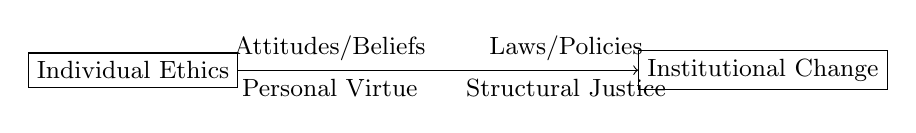
\begin{tikzpicture}
				\small
				\node (individual) at (-1,0) [draw, rectangle] {Individual Ethics};
				\node (institutional) at (7,0) [draw, rectangle] {Institutional Change};
				\draw [->] (individual) -- (institutional);
				
				\node [below] at (1.5,0) {Personal Virtue};
				\node [below] at (4.5,0) {Structural Justice};
				
				\node [above] at (1.5,0) {Attitudes/Beliefs};
				\node [above] at (4.5,0) {Laws/Policies};
			\end{tikzpicture}
		\end{center}
	\end{frame}
	
	\begin{frame}{What Are We Ethically Allowed to Do? Limits of Racial Justice Work}
		\begin{itemize}
			\item Ethical means must align with ethical ends in pursuing racial justice.
			\item Constitutional democracy places legal constraints on certain forms of racial justice activism.
			\item \textbf{Proportionality} requires that actions taken match the severity of the injustice being addressed.
			\item Different philosophical traditions offer different answers about permissible tactics for fighting injustice.
		\end{itemize}
		
		\begin{exampleblock}{Ethical Considerations in Racial Justice Activism}
			\begin{tabular}{|l|l|}
				\hline
				\textbf{Ethical Question} & \textbf{Considerations} \\
				\hline
				Civil Disobedience & When is breaking unjust laws justified? \\
				Truth Commissions & Balancing truth-telling with reconciliation \\
				Reparations & Determining fair compensation for historical wrongs \\
				Speech Restrictions & Weighing harm prevention against free expression \\
				\hline
			\end{tabular}
		\end{exampleblock}
	\end{frame}
	
	

\end{document}